\begin{figure}[p]
    \centering
    \begin{subfigure}{0.47\linewidth}
        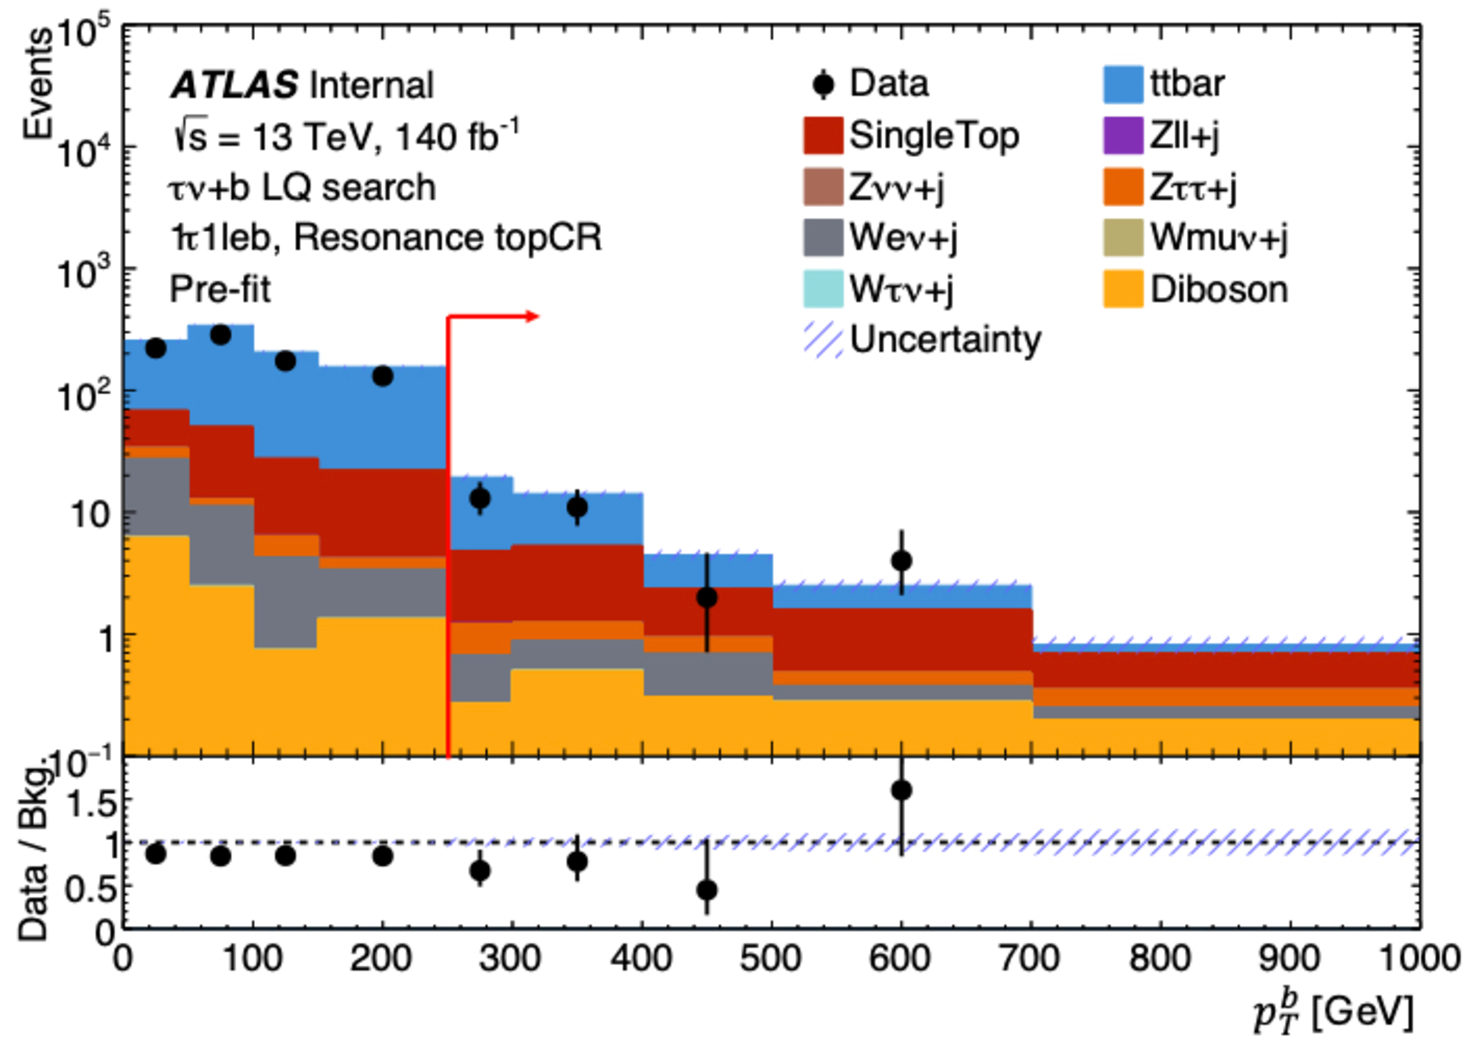
\includegraphics[width=\linewidth]{Figs/CH8/TopCR_ele_Res_bjet_pT.pdf}
        \caption[]{$\pT^b$, $e$ channel}
    \end{subfigure}\hfill
    \begin{subfigure}{0.47\linewidth}
        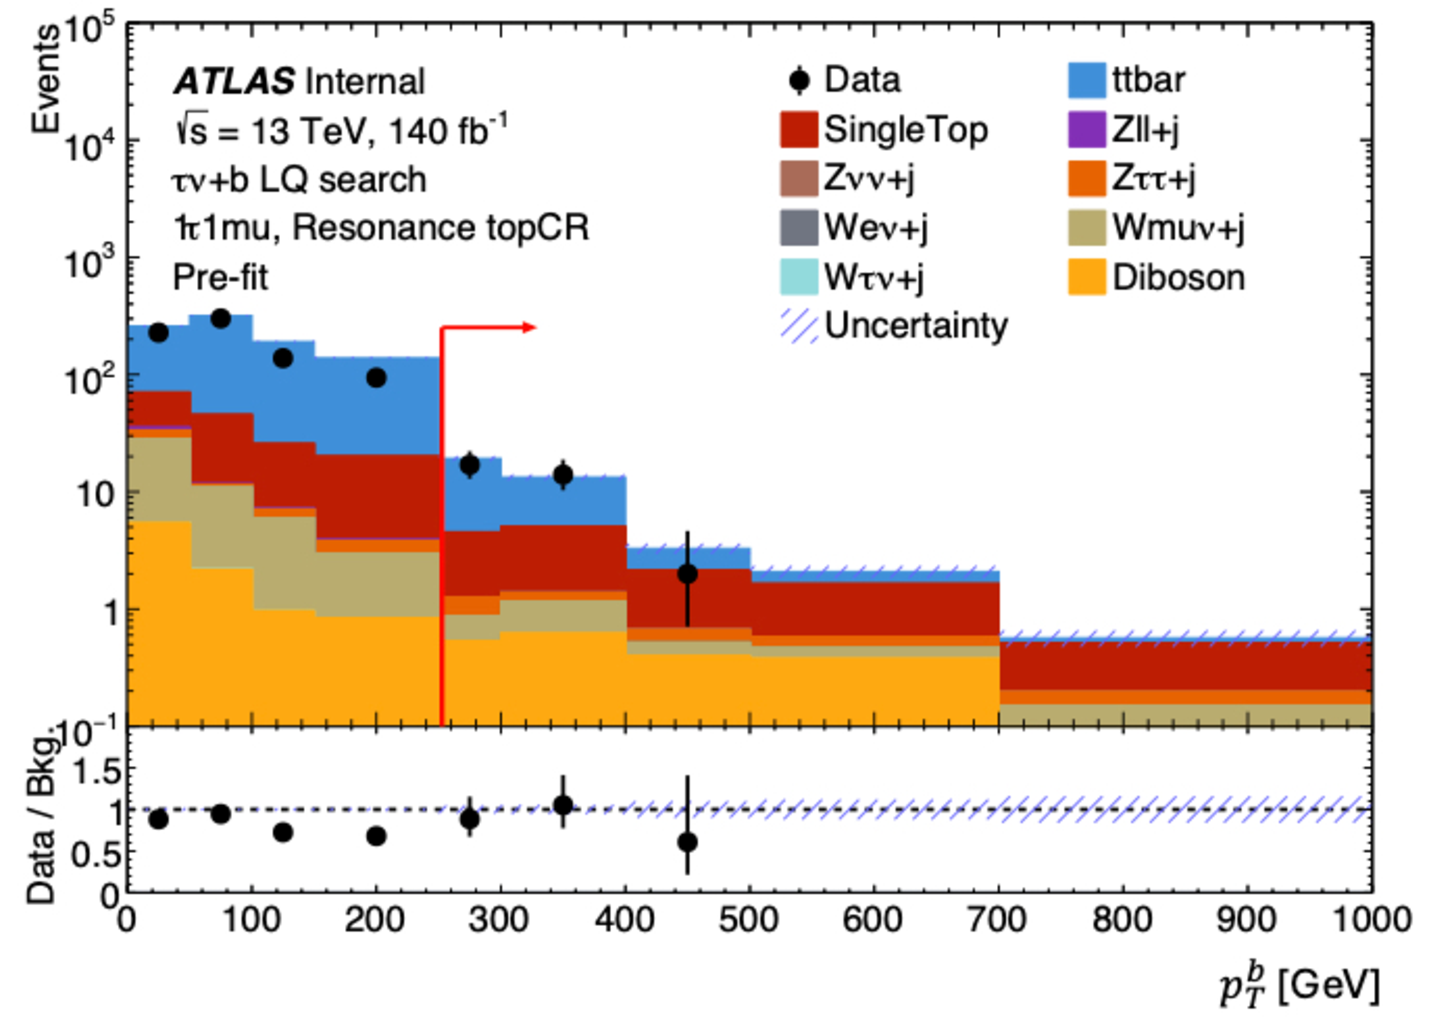
\includegraphics[width=\linewidth]{Figs/CH8/TopCR_mu_Res_bjet_pT.pdf}
        \caption[]{$\pT^b$, $\mu$ channel}
    \end{subfigure}\par\medskip
    \begin{subfigure}{0.47\linewidth}
        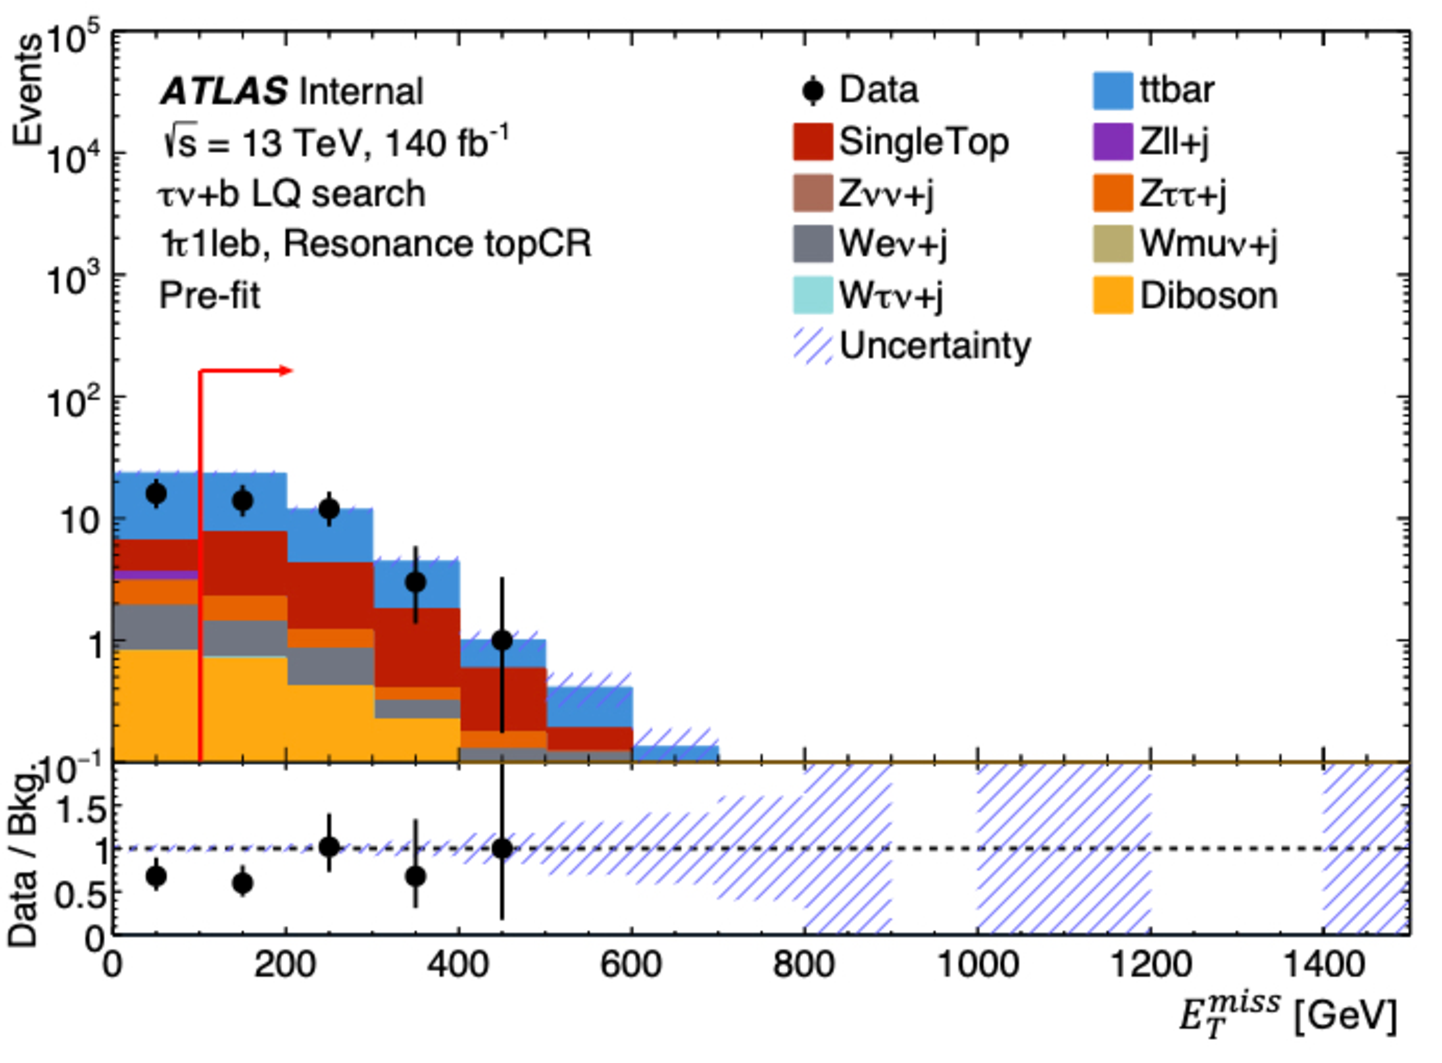
\includegraphics[width=\linewidth]{Figs/CH8/TopCR_ele_Res_met.pdf}
        \caption[]{$\met$, $e$ channel}
    \end{subfigure}\hfill
    \begin{subfigure}{0.47\linewidth}
        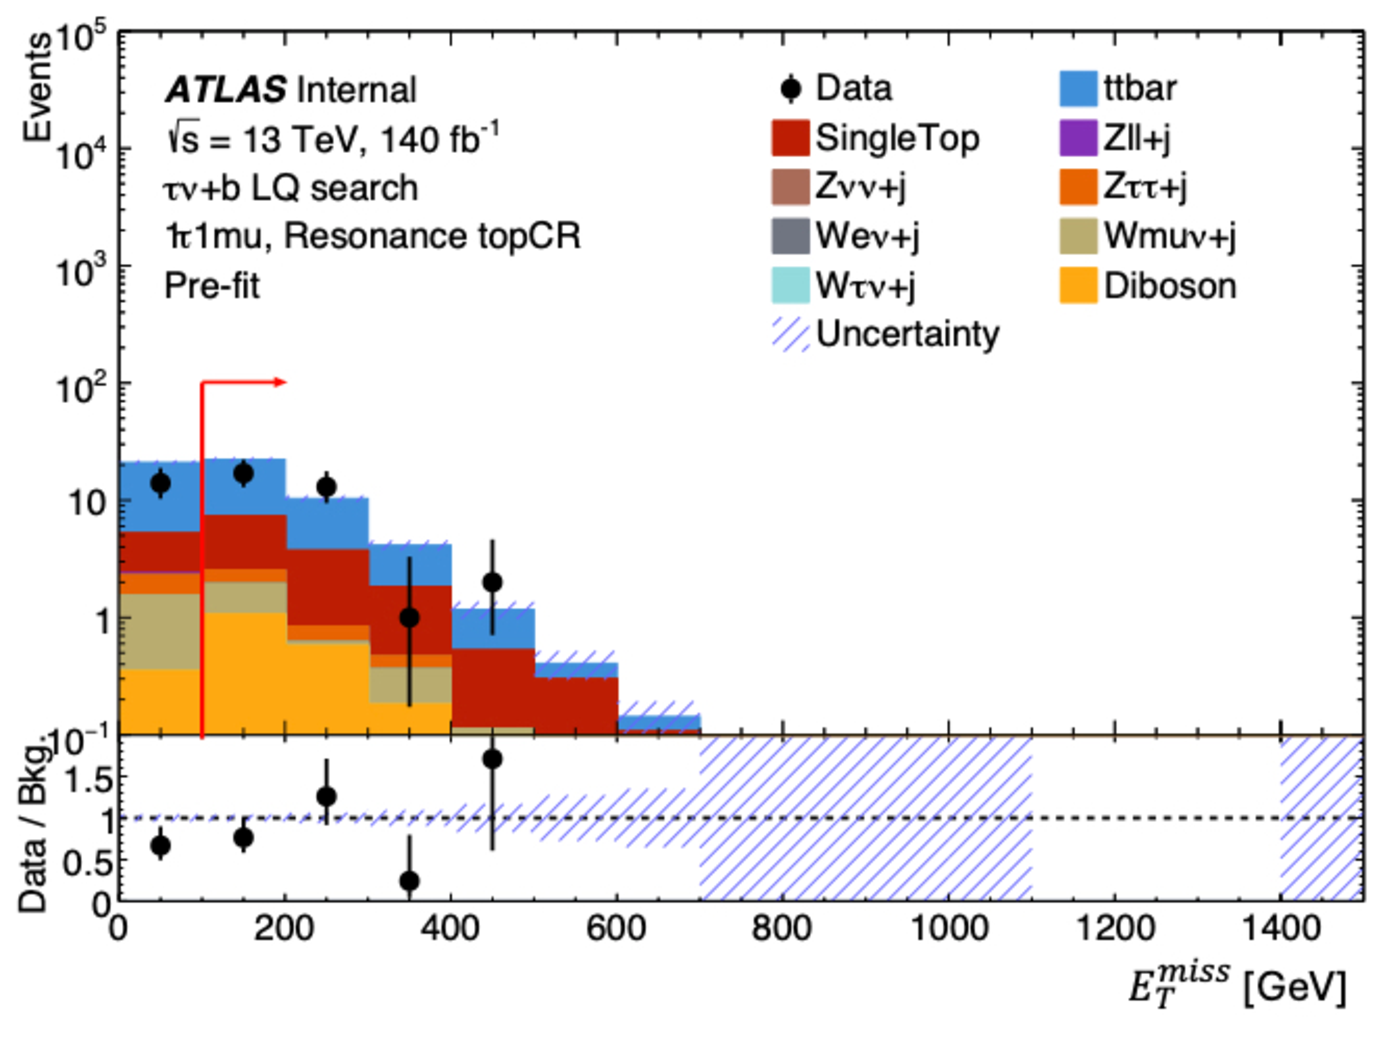
\includegraphics[width=\linewidth]{Figs/CH8/TopCR_mu_Res_met.pdf}
        \caption[]{$\met$, $\mu$ channel}
    \end{subfigure}\par\medskip
    \begin{subfigure}{0.47\linewidth}
        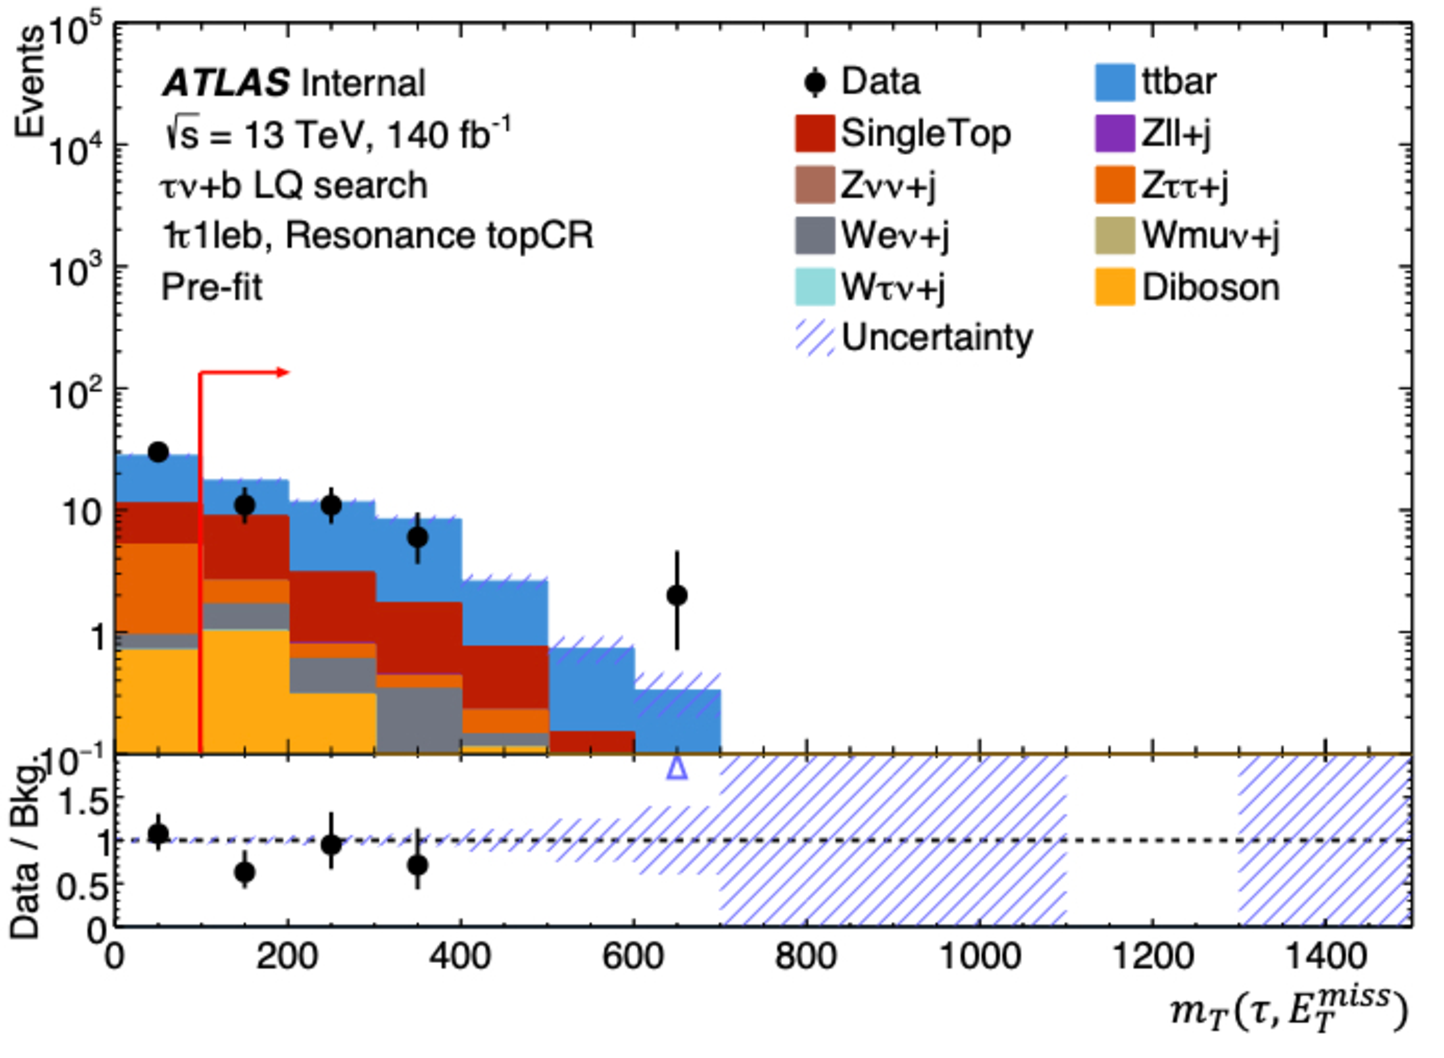
\includegraphics[width=\linewidth]{Figs/CH8/TopCR_ele_Res_mT.pdf}
        \caption[]{$\mT$, $e$ channel}
    \end{subfigure}\hfill
    \begin{subfigure}{0.47\linewidth}
        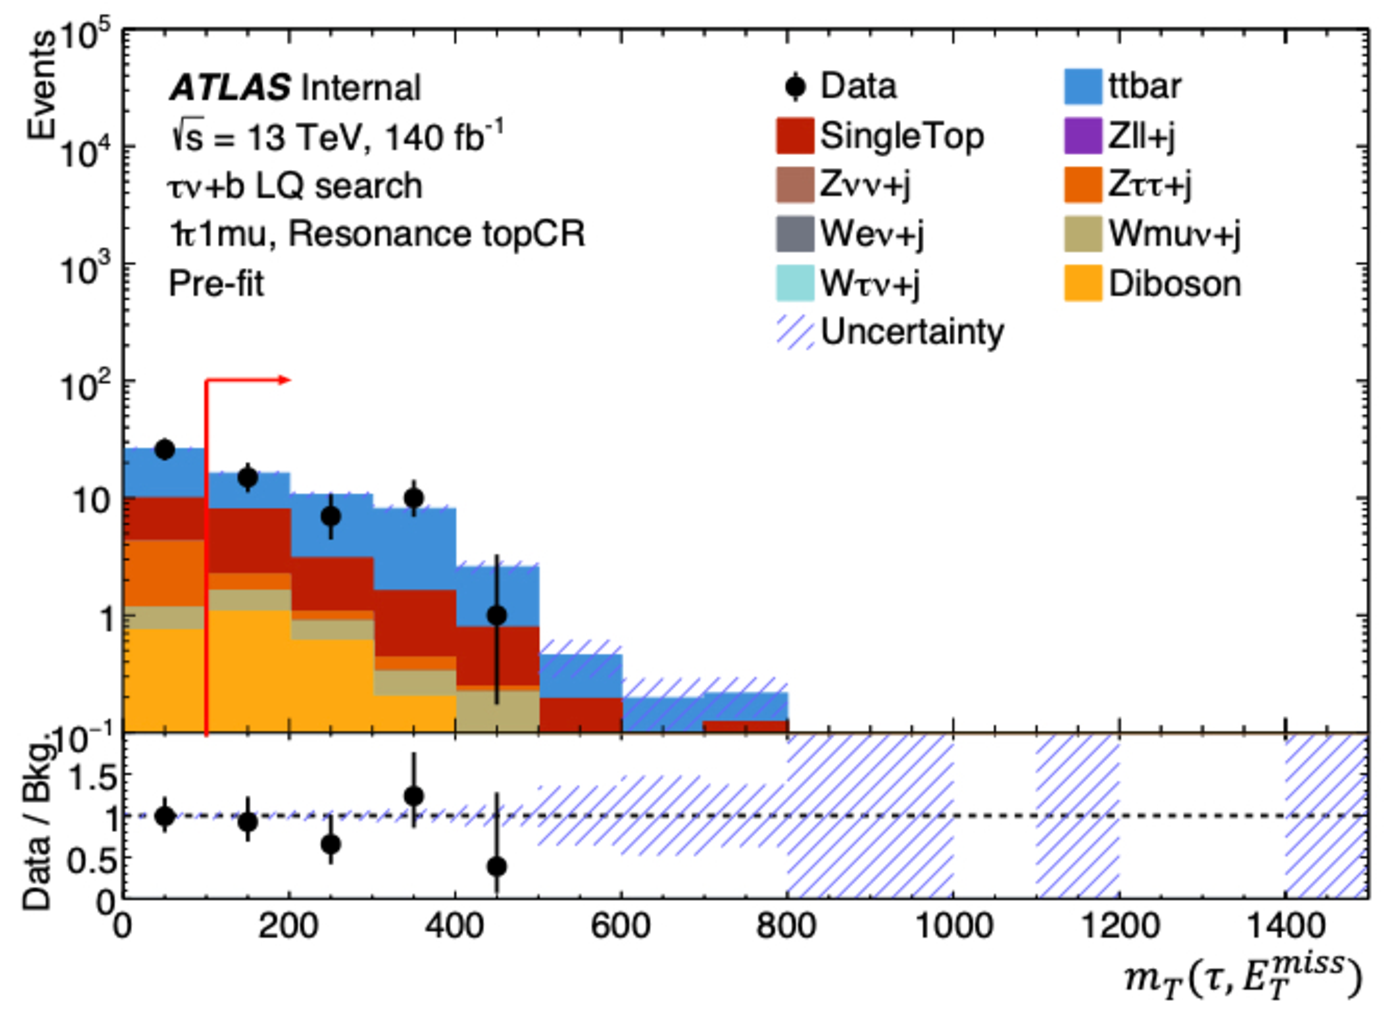
\includegraphics[width=\linewidth]{Figs/CH8/TopCR_mu_Res_mT.pdf}
        \caption[]{$\mT$, $\mu$ channel}
    \end{subfigure}\par\medskip
    \caption[Pre-fit N-1 distributions in CRTop-Res]{Pre-fit $N-1$ distributions in CRTop-Res, with the electron channel in the left column and the muon channel in the right column. The stacked prediction contains all simulated backgrounds. The lower panels show data divided by the total prediction, and the hatched bands show the statistical uncertainty in that prediction. Arrows indicate the selection boundaries. The last bin includes the overflow.}
    \label{fig:ch8_topcr_res}
\end{figure}

\begin{figure}[p]
    \centering
    \begin{subfigure}{0.47\linewidth}
        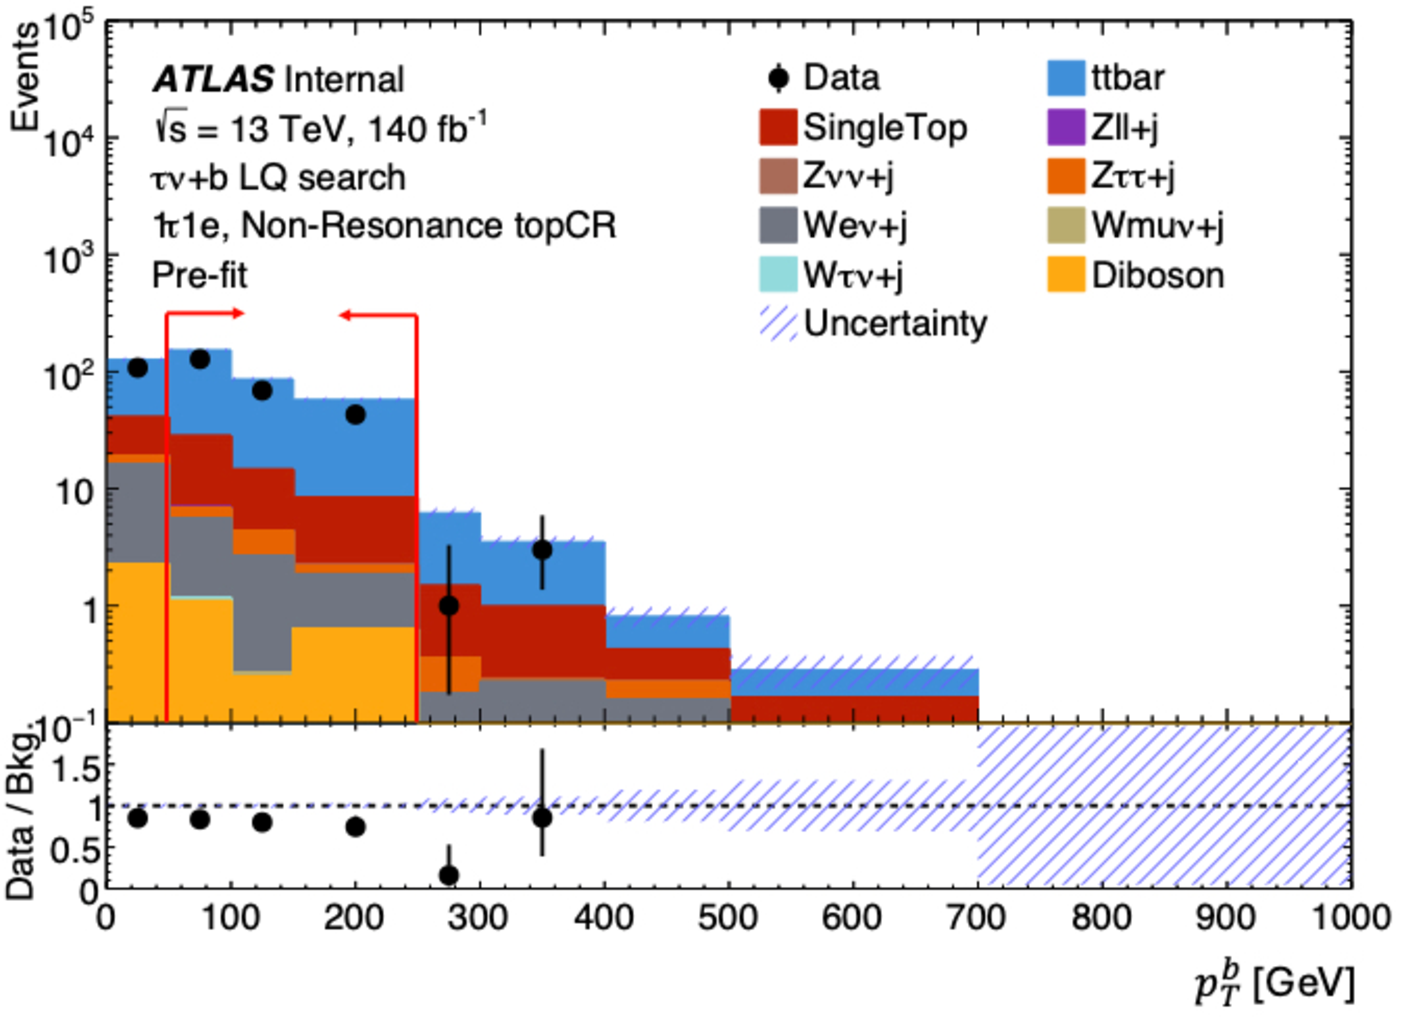
\includegraphics[width=\linewidth]{Figs/CH8/TopCR_ele_NonRes_bjet_pT.pdf}
        \caption[]{$\pT^b$, $e$ channel}
    \end{subfigure}\hfill
    \begin{subfigure}{0.47\linewidth}
        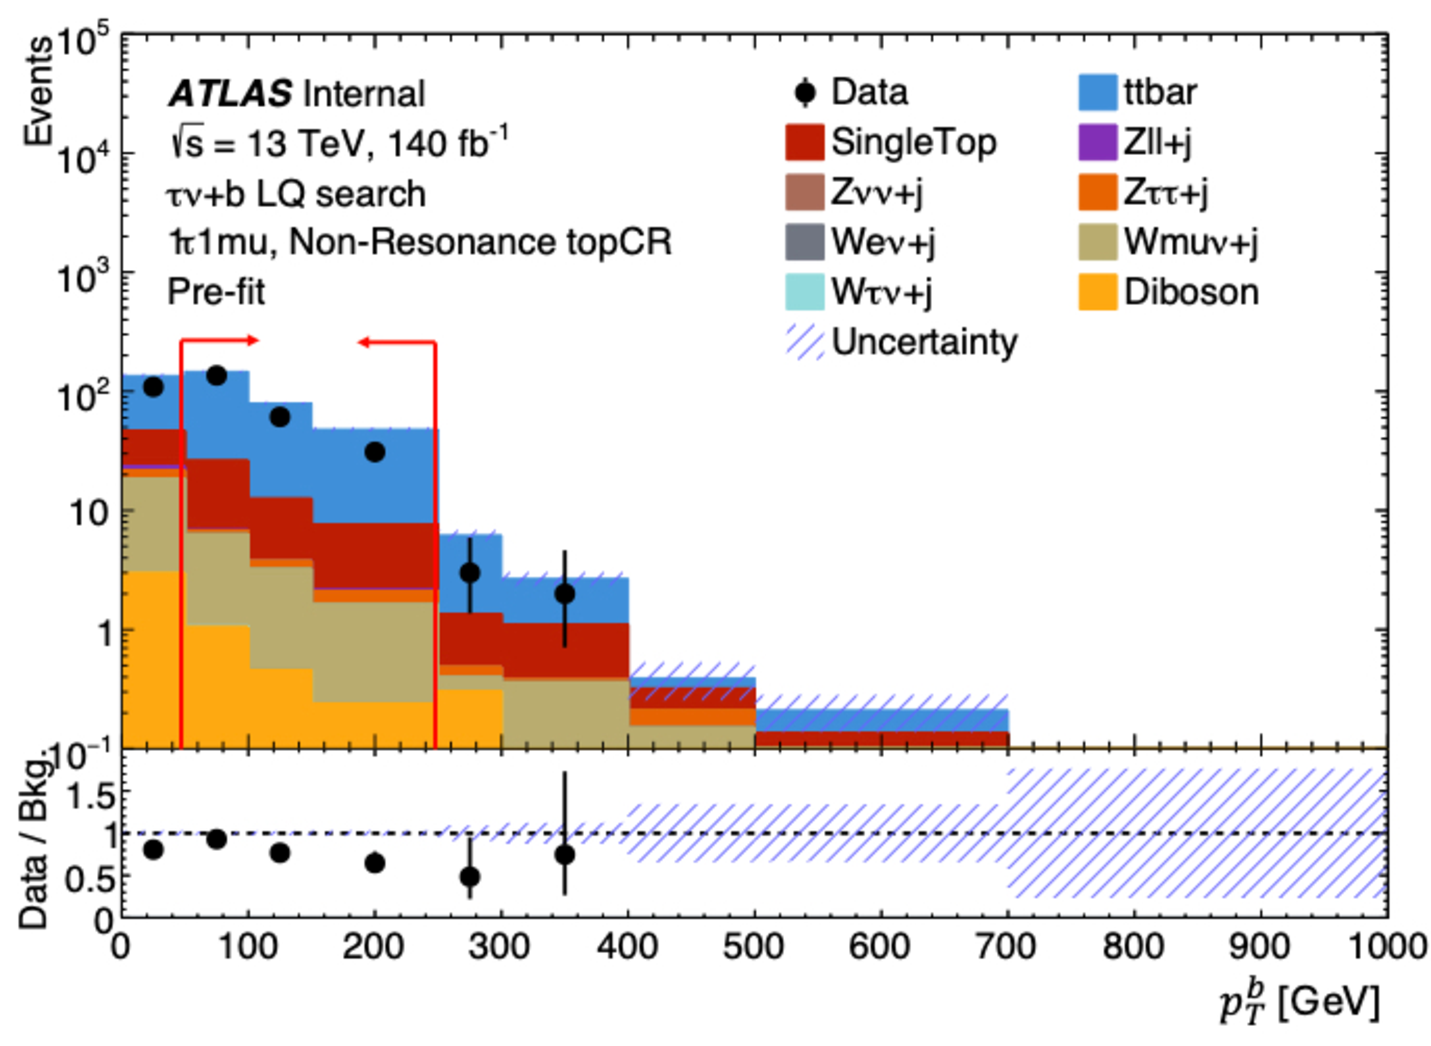
\includegraphics[width=\linewidth]{Figs/CH8/TopCR_mu_NonRes_bjet_pT.pdf}
        \caption[]{$\pT^b$, $\mu$ channel}
    \end{subfigure}\par\medskip
    \begin{subfigure}{0.47\linewidth}
        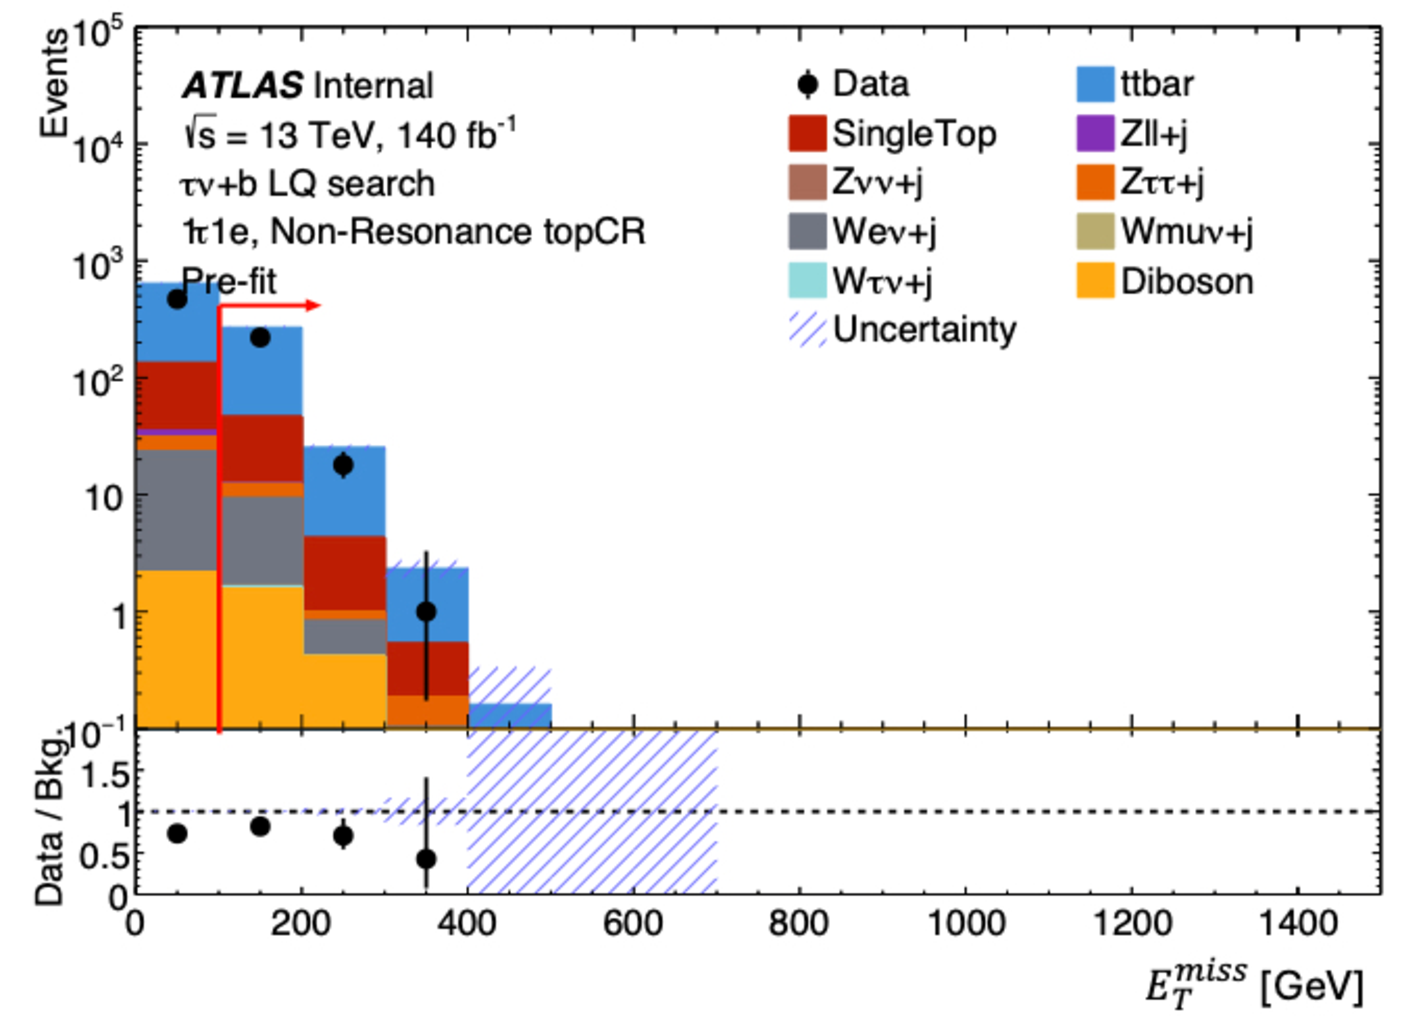
\includegraphics[width=\linewidth]{Figs/CH8/TopCR_ele_NonRes_met.pdf}
        \caption[]{$\met$, $e$ channel}
    \end{subfigure}\hfill
    \begin{subfigure}{0.47\linewidth}
        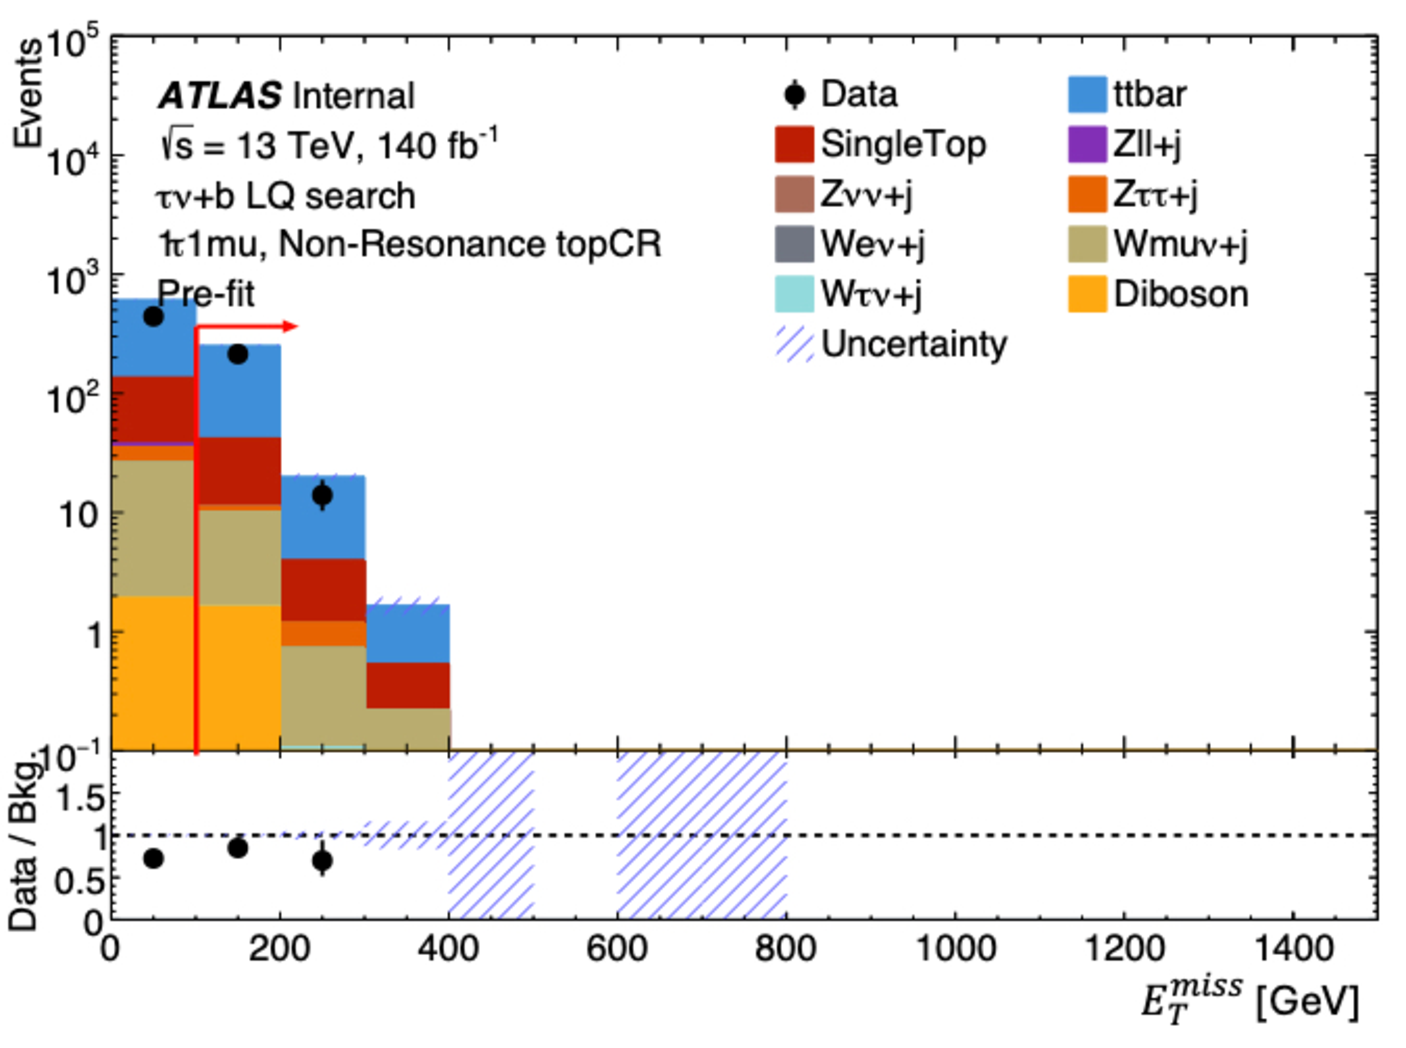
\includegraphics[width=\linewidth]{Figs/CH8/TopCR_mu_NonRes_met.pdf}
        \caption[]{$\met$, $\mu$ channel}
    \end{subfigure}\par\medskip
    \begin{subfigure}{0.47\linewidth}
        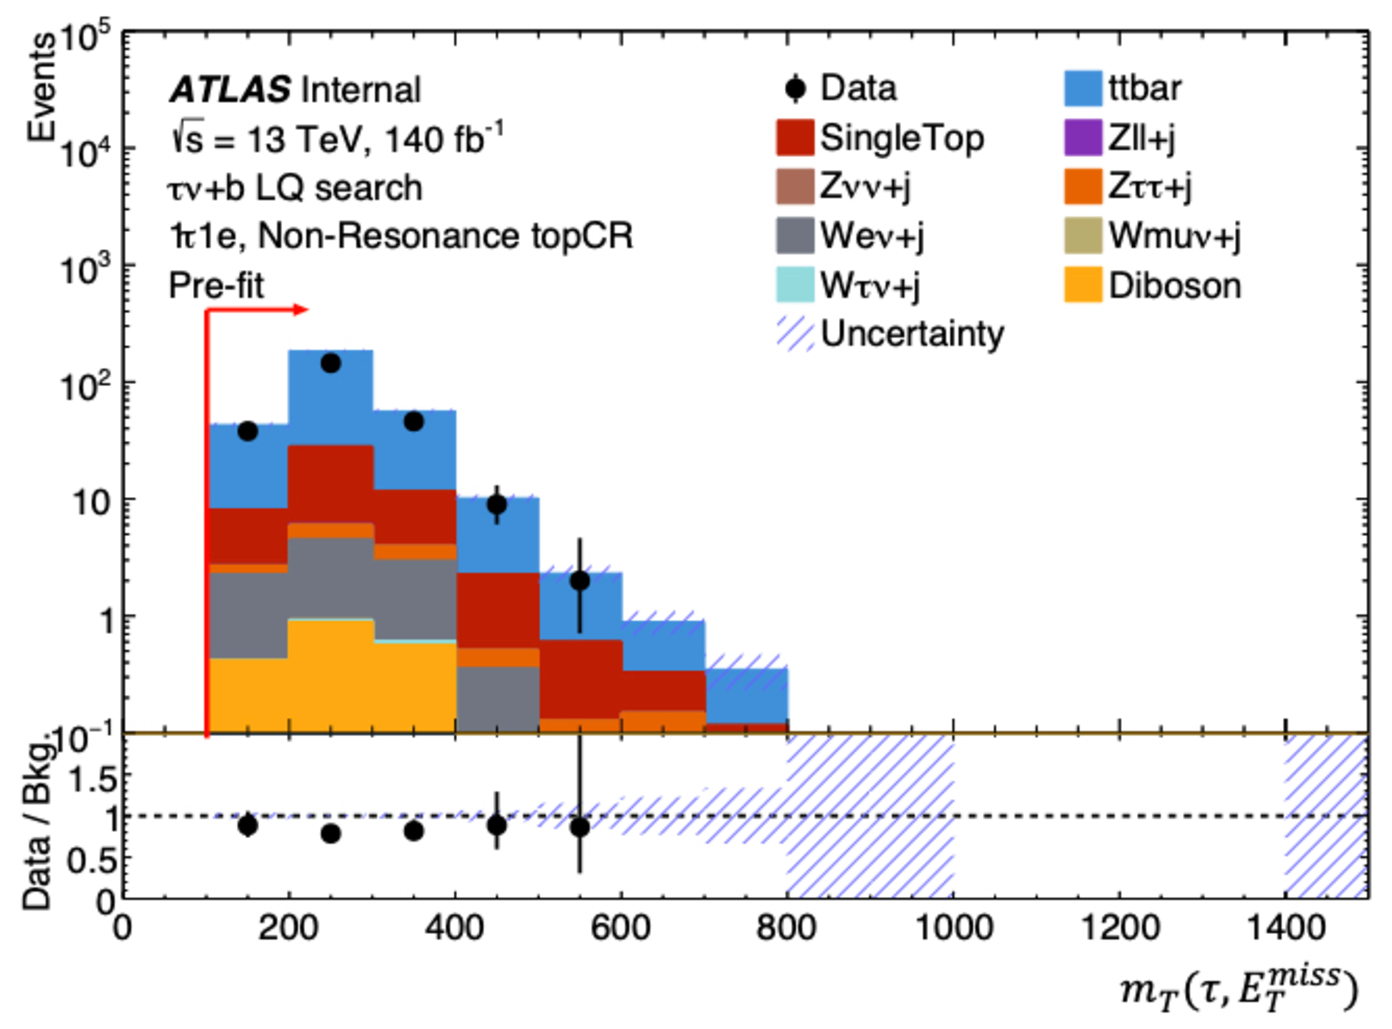
\includegraphics[width=\linewidth]{Figs/CH8/TopCR_ele_NonRes_mT.pdf}
        \caption[]{$\mT$, $e$ channel}
    \end{subfigure}\hfill
    \begin{subfigure}{0.47\linewidth}
        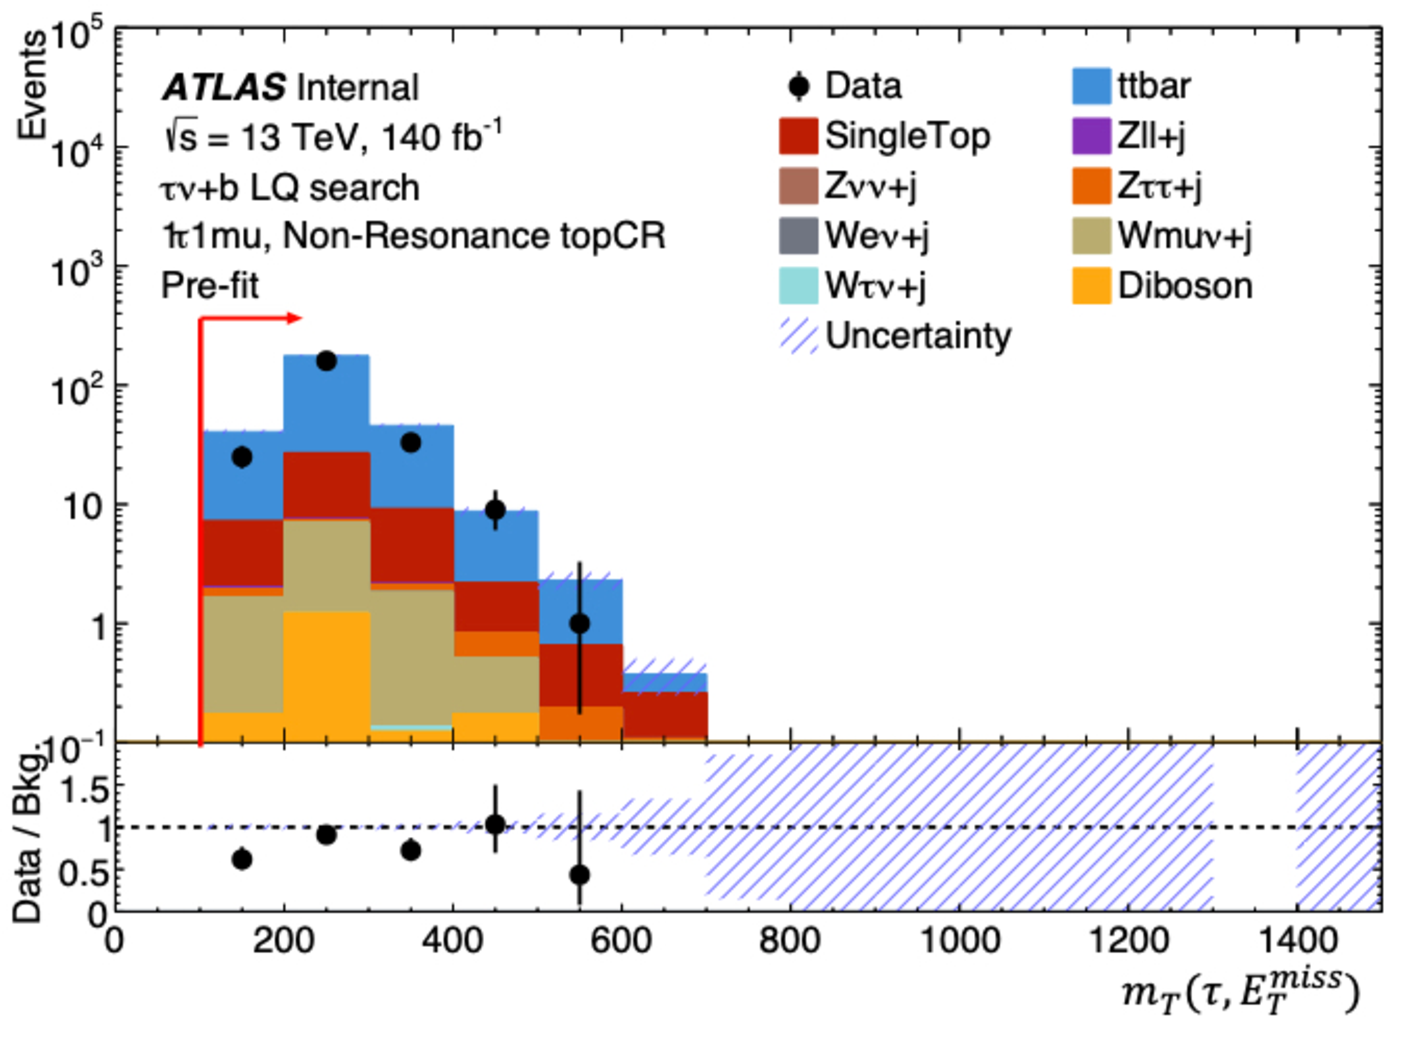
\includegraphics[width=\linewidth]{Figs/CH8/TopCR_mu_NonRes_mT.pdf}
        \caption[]{$\mT$, $\mu$ channel}
    \end{subfigure}\par\medskip
    \caption[Pre-fit N-1 distributions in CRTop-NonRes]{Pre-fit $N-1$ distributions in CRTop-NonRes, with the electron channel in the left column and the muon channel in the right column. The stacked prediction contains all simulated backgrounds. The lower panels show data divided by the total prediction, and the hatched bands show the statistical uncertainty in that prediction. Arrows indicate the selection boundaries. The last bin includes the overflow.}
    \label{fig:ch8_topcr_nonres}
\end{figure}
